\documentclass[1-ambra-tesi.tex]{subfiles}
 
\begin{document}
\label{sub:CTA}

\begin{chapabstract}
\small{\lipsum[1]}\\

\begin{center}
    \noindent\makebox[0.8\linewidth]{\rule{0.8\paperwidth}{0.4pt}}
\end{center}
\vspace{2cm}
\end{chapabstract}

% ============================ MONKEYS ==============================

\lipsum[2]

\section{Let's talk about monkeys}
\label{sec:monkeys}
\lipsum[3]

% multiple figure example
\begin{figure}[ht]
    \centering
    \begin{subfigure}[l]{0.45\linewidth}
    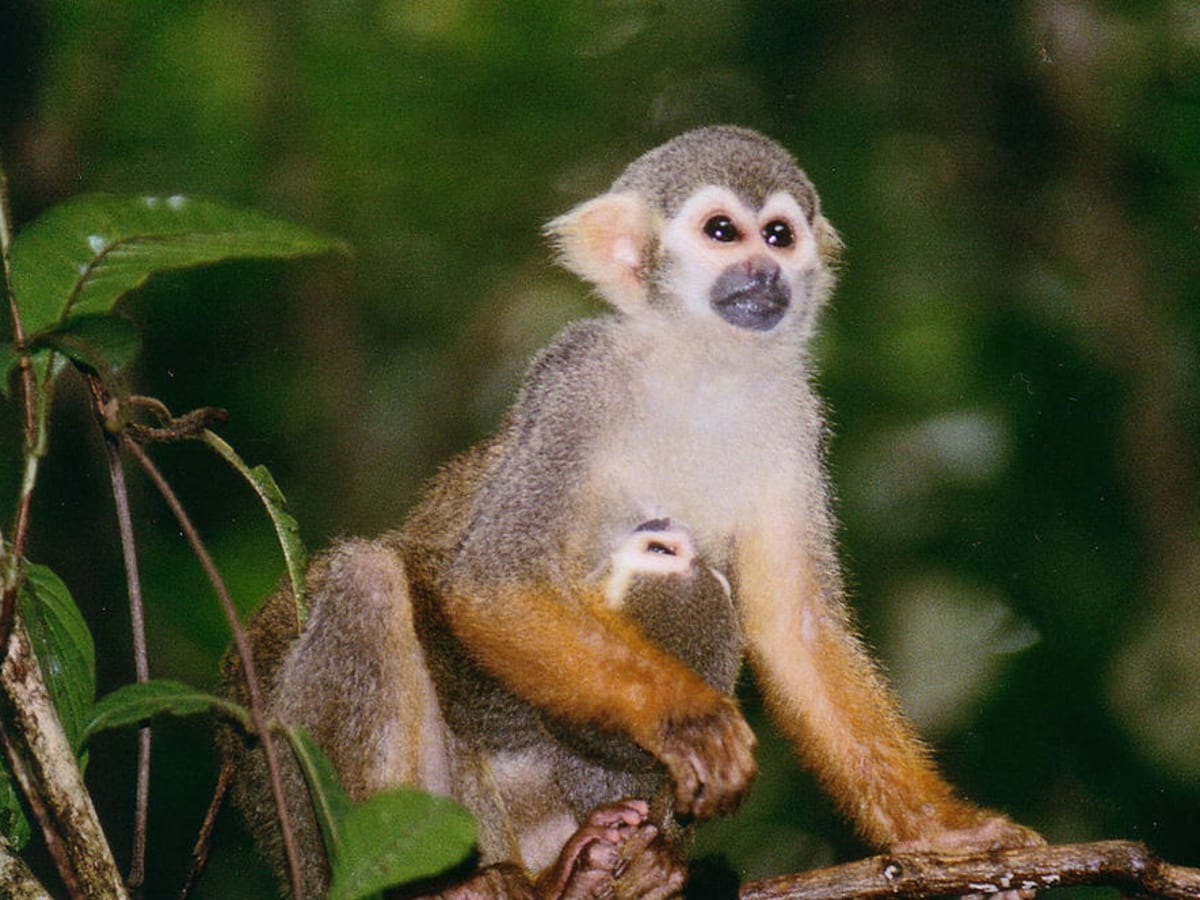
\includegraphics[width=\linewidth]{images/monkeys.jpeg}
    \caption{}
    \end{subfigure}
    \begin{subfigure}[r]{0.51\linewidth}
    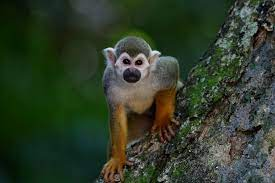
\includegraphics[width=\linewidth]{images/monkeys2.jpeg}
    \caption{}
    \end{subfigure}
    \caption{\textbf{Left} A cute monkey. \textbf{Right} Another cute monkey. \textbf{Credits:} the web (left), the web (right).}
    \label{fig:monkeys}
\end{figure}

\lipsum[4] \\

Referring to introduction: \ref{sec:intro}.\\

\lipsum[5]\\

Quoting the image: \ref{fig:monkeys}.\\

\lipsum[6]



\end{document}

